\section{Differentiation in $\reals^n$}

Recall the definition of a one-dimensional derivative: 

\definition{One dimensional derivative}{
    Let $\Omega\subseteq\reals$ be open, and $f:\Omega\to \reals$. We say $f$ is \textbf{differentiable} at $x_0\in\Omega$ if the limit \[
    \lim_{x\to x_0} \frac{f(x)-f(x_0)}{x-x_0}
    \]
    exists, and we call this the \textbf{derivative} of $f$ at $x_0$, and denote it $f'(x_0)$.
}
It is a bit hard to extend this definition to functions $\reals^n\to\reals^m$. Let $\vec{f}:\reals^n\to\reals^m$, we forcefully write \begin{align*}
    \vec{f}'(\vec{x}_0) =\lim_{\vec{x}\to\vec{x}_0}\frac{\vec{f}(\vec{x})-\vec{f}(\vec{x}_0)}{\vec{x}-\vec{x}_0},
\end{align*}
this equation does not really make sense, as we do not have a way to divide by a vector.
There are two ways to mitigate this. The first way is to compress everything into one-dimension, and take the derivative with respect to one variable while holding all others constant.
\definition{Partial Derivative}{
    Let $\Omega\subseteq\reals^n$, and $f:\Omega\to\reals^m$. For $1\leq k \leq n$, we say the \textbf{partial derivative} of $f$ with respect to $x_k$ at $\vec{a}\in \Omega$ is the limit \[
    \lim_{\tilde{a}_k\to a_k} \frac{f(a_1,\ldots,\tilde{a}_k,\ldots, a_n)-f(a_1,\ldots,a_k,\ldots, a_n)}{\tilde{a}_k - a_k}. 
    \]
    In other words, this is the one-dimensional derivate in the variable $x_k$.
}
\begin{notation}
The partial derivative is denoted \[
\frac{\partial f}{\partial x_k}(\vec{a})\textrm{\quad or \quad }f_{x_k}(\vec{a}).
\]
\end{notation}

\example{
    Let $f(x,y)=(2x+\sin(xy),-y+\cos(xy))$. Compute the partial derivatives of $f$ in $x$ and $y$.
}
To compute the partial derivative in $x$ (resp. $y$), we hold $y$ constant, so under constant $y$ (resp. $x$), \begin{align*}
    \frac{\partial f}{\partial x} (x,y) =& (2+y\cos(xy), -y\sin (xy)),\\
    \frac{\partial f}{\partial y} (x,y) =& (x\cos(xy),-x\sin(xy)).
\end{align*}

The existence of a partial derivative implies the existence of a total derivative, so let us try to motivate the definition of that `real derivative'.
Rethinking the one-dimensional derivative, we also use the derivative $f'(x_0)$ as a linear approximation for the function $f$. What this means is that for small $\Delta x$, \[
f(x_0+\Delta x) = f(x_0)+ f'(x_0)\Delta x + \textrm{small error}.
\]
How small is this error? Moving everything else to one side and taking the limit $\Delta x\to 0$, \begin{align*}
    \lim_{\Delta x \to 0 }\left|\frac{\textrm{small error}}{\Delta x}\right| &= \lim_{\Delta x \to 0 }\frac{f(x_0+\Delta x) - f(x_0)- f'(x_0)\Delta x}{\Delta x}\\
    &=\lim_{\Delta x \to 0 }\frac{f(x_0+\Delta x) - f(x_0)}{\Delta x} - f'(x_0)\\
    &=f'(x_0)-f'(x_0)\\
    &=0.
\end{align*}
This means our error using this linear approximation shrinks faster $\Delta x$. Thus, we say that this is the best linear approximation for functions, and visually represent it as the line tangent to the curve at the point $(x_0,f(x_0))$.
Similarly, we ask in higher dimensions, if we can approximate a function to be `locally linear', i.e. there is a linear transformation \begin{align*}
    \vec{f}(\vec{x_0}+\Delta \vec{x}) = \vec{f(x_0)}+  T(\Delta \vec{x}) + \textrm{small error},
\end{align*}
with this small error shrinking to $\vec{0}$ faster than $\Delta \vec{x}$, or \[
\lim_{\Delta \vec{x}\to \vec{0}} \frac{|\textrm{small error}|}{|\Delta \vec{x}|}=0.
\]
If there is such a transformation $T:\reals^n\to\reals^m$, then $T$ should be the higher dimensional `derivative' of $\vec{f}$ at $\vec{x}_0$. 
By the Matrix Representation of Linear Transformations, let us write the derivative $T$ as a matrix. \definition{Total Derivative}{
    \domain{\vec{f}}{n}{m}. We say $f$ is differentiable at $\vec{x}_0\in\Omega$ if there is $A\in M_{m\times n}$ such that \[
    \lim_{\vec{x}\to\vec{x}_0} \frac{\vec{f}(\vec{x})-\vec{f}(\vec{x}_0)-A(\vec{x}-\vec{x}_0)}{|\vec{x}-\vec{x}_0|} =\vec{0}.
    \]
    In this case, we call $A$ the \textbf{(total) derivative} of $\vec{f}$ at $\vec{x}_0$, and denote it $d\vec{f}|_{\vec{x}_0}$.
}
\theorem{Differentiable functions are continuous}{
    \domain{f}{n}{m} be differentiable everywhere on $\Omega$. Then $f$ is continuous.
    
}
\begin{proof}
    Let $\vec{x}_0\in\Omega$. We have 
    \[
    \lim_{\vec{x}\to\vec{x}_0} \frac{\vec{f}(\vec{x})-\vec{f}(\vec{x}_0)-df|_{\vec{x}_0}(\vec{x}-\vec{x}_0)}{|\vec{x}-\vec{x}_0|} =\vec{0},
    \]
    and want to show \[
        \lim_{\vec{x}\to\vec{x}_0} \vec{f}(\vec{x})-\vec{f}(\vec{x}_0)=\vec{0}.
    \]
    Here we apply a standard trick (plus-minus), which means we massage the second equation to resemble the first:\begin{align*}
        \lim_{\vec{x}\to\vec{x}_0} \vec{f}(\vec{x})-\vec{f}(\vec{x}_0) &= \lim_{\vec{x}\to\vec{x}_0} \vec{f}(\vec{x})-\vec{f}(\vec{x}_0)-df|_{\vec{x}_0}(\vec{x}-\vec{x}_0)-df|_{\vec{x}_0}(\vec{x}-\vec{x}_0)\\
        &=\lim_{\vec{x}\to\vec{x}_0} \frac{\vec{f}(\vec{x})-\vec{f}(\vec{x}_0)-df|_{\vec{x}_0}(\vec{x}-\vec{x}_0)}{|\vec{x}-\vec{x}_0|} |\vec{x}-\vec{x}_0|-df|_{\vec{x}_0}(\vec{x}-\vec{x}_0)\\
    \end{align*}
    The first term is $\vec{0}*0 $ by the definition of derivative, and $|\vec{x}-\vec{x}_0|$ is a composition of elementary functions thus continuous. The second term is $df|_{\vec{x}_0}(\vec{0})$ as linear transformations are polynomials thus continuous.
    Therefore the whole expression equals $\vec{0}$.
\end{proof}
\theorem{Uniqueness of derivative}{
    The derivative $df$, if it exists, is unique and equals the matrix \begin{equation*}
        J = \begin{bmatrix}
            \frac{\partial \vec{f}}{\partial x_1} &
            \frac{\partial \vec{f}}{\partial{x}_2} &
            \frac{\partial \vec{f}}{\partial {x}_3} &
            \ldots&
            \frac{\partial \vec{f}}{\partial {x}_n}
        \end{bmatrix}
    \end{equation*}
    evaluated at $\vec{x}_0$.
}
\definition{Jacobian Matrix}{
    Suppose the partial derivatives of $\vec{f}$ exist, then we call the matrix 
        \begin{equation*}
            J  \begin{bmatrix}
                \frac{\partial \vec{f}}{\partial x_1} &
                \frac{\partial \vec{f}}{\partial{x}_2} &
                \frac{\partial \vec{f}}{\partial {x}_3} &
                \ldots&
                \frac{\partial \vec{f}}{\partial {x}_n}
            \end{bmatrix}=
        \end{equation*}
    
    the \textbf{Jacobian Matrix} of $f$.
}
Before we go on to the proof, try if you can prove this using the ideas from the Matrix Representation of a linear transformation.
Here is a hint: The partial derivative can also be written as \[
\frac{\partial{f}}{\partial {x}_k}(\vec{x}_0) = \lim_{h\to 0}\frac{f(\vec{x}_0+h\vec{e}_k)-f(\vec{x}_0)}{h}.
\]
\begin{proof}[Proof of Uniqueness of Derivative]
    Let $\vec{x}_0\in \Omega$. By the uniqueness of limit, we approach the limit \[
        \lim_{\vec{x}\to\vec{x}_0} \frac{\vec{f}(\vec{x})-\vec{f}(\vec{x}_0)-d\vec{f}|_{\vec{x}_0}(\vec{x}-\vec{x}_0)}{|\vec{x}-\vec{x}_0|}
    \]
    along the line $\vec{x}=\vec{x}_0+h\vec{e}_k$ as $h\to 0$. Therefore, 
    \begin{align*}
        &\lim_{h\to 0} \frac{\vec{f}(\vec{x}_0+h\vec{e}_k)-\vec{f}(\vec{x}_0)-d\vec{f}|_{\vec{x}_0}(h\vec{e}_k)}{|h|}=\vec{0} \\
        \implies &\lim_{h\to 0} \frac{\vec{f}(\vec{x}_0+h\vec{e}_k)-\vec{f}(\vec{x}_0)-d\vec{f}|_{\vec{x}_0}(h\vec{e}_k)}{h}=\vec{0}\\
        \implies &\lim_{h\to 0} \frac{\vec{f}(\vec{x}_0+h\vec{e}_k)-\vec{f}(\vec{x}_0)}{h}-d\vec{f}|_{\vec{x}_0}(\vec{e}_k)=\vec{0}.\\
    \end{align*}
    This means that the $k$-th column of $d\vec{f}|_{\vec{x}_0}$ is $\vec{f}_{x_k}(\vec{x}_0)$, the partial derivative of $\vec{f}$ with respect to the $k$-th variable.
\end{proof}

\corollary{
    If a function has a total derivative, then its partial derivatives exist.
}

\example{
    Determine if the function \[
    f(x,y)= x^2+y^2.
    \]
    is differentiable.
}
If this function is differentiable then the derivative must be the Jacobian $[2x \ 2y]$. Indeed, we can check for every $(x_0,y_0)\in\reals^2$ \begin{align*}
    &\lim_{(x,y)\to(x_0,y_0)}\frac{x^2+y^2-x_0^2-y_0^2 - \begin{bmatrix}
        2x_0 & 2y_0 
    \end{bmatrix}\begin{bmatrix}
        (x-x_0)\\(y-y_0)
    \end{bmatrix}}{|(x,y)-(x_0,y_0)|}\\
    =&\lim_{(x,y)\to(x_0,y_0)}\frac{
        (x-x_0)^2+(y-y_0)^2}{((x-x_0)^2+(y-y_0)^2)^{1/2}}\\
    =&0.
\end{align*}
Therefore, this function is differentiable everywhere in $\reals^2$.

Having partial derivatives is not a sufficient condition for differentiability.
\example{
    Compute the partial derivatives of the function \[
    f(x,y)=\begin{cases}
        \frac{xy}{x^2+y^2}, &\textrm{ if }(x,y)\neq (0,0)\\
        0, &\textrm{ if }(x,y)=0,0
    \end{cases}
    \]
    at $(x,y)=0,0$.
}
The partial derivatives in $x$ and $y$ are both $0$, as $f=0$ when $x=0$ or $y=0$. However, this function is not differentiable. You can show this by checking that the Jacobian matrix $J$ does not satisfy the definition of the derivative. We can also get by with less work. This function is not even continuous! In fact, if we approach the limit $(x,y)\to(0,0)$ along $y=x$,
we get \[
\lim_{x\to 0 }\frac{x^2}{x^2+x^2} = \frac{1}{2}\neq f(0,0).
\]
\example{
    Determine if the function \[
    f(x,y)=\begin{cases}
        \frac{2x^2y+y^3}{x^2+y^2}, &\textrm{ if }(x,y)\neq (0,0)\\
        0, &\textrm{ if }(x,y)=0,0
    \end{cases}
    \]
    is differentiable at $(x,y)=0,0$.
}
This function is continuous at $(0,0)$. Indeed we have \begin{align*}
    f_x(0,0) = 0, f_y(0,0)= \lim_{y\to 0 } \frac{1}{y}\frac{y^3}{y^2}=1.
\end{align*}
Now let us investigate the limit \begin{align*}
    \lim_{(x,y)\to(0,0)}\frac{\frac{2x^2y+y^3}{x^2+y^2} - \begin{bmatrix}
        0&1
    \end{bmatrix}\begin{bmatrix}
        x\\y
    \end{bmatrix}}{\sqrt{x^2+y^2}}
    =\lim_{(x,y)\to(0,0)}\frac{2x^2y+y^3-x^2y-y^3}{(x^2+y^2)^{3/2}}=
    \lim_{(x,y)\to(0,0)}\frac{x^2y}{(x^2+y^2)^{3/2}}.
\end{align*}
This limit does not exist. Specifically, the limit as we approach along the $x$-axis is $0$, but is not zero if we take the limit along the line $x=y$. Therefore this function is not differentiable at $(0,0)$.

\theorem{Differentiability}{
    \domain{f}{n}{m}. Let $x_0\in\Omega$, and the partial derivatives of $f$ are continuous in some open ball $B(x_0,\epsilon)\subseteq \Omega$. Then $f$ is differentiable at $x_0$.
}
The proof is optional. Here is the idea: Since we compute limit of vectors as the limit in each coordinate, it suffices to check that each component of $f= (f_1,f_2,\ldots, f_m)$ is differentiable. Now let us restrict to one of these $f_i$'s, and call it $g$. We already have a candidate for its derivative, namely we want to show \[
    Dg(\vec{x}) = \begin{bmatrix}
        \pdv{g}{x_1}(\vec{x}) & \cdots & \pdv{g}{x_n}(\vec{x})
    \end{bmatrix}.
\]
Let us consider a point $\vec{x}+\vec{h}$. We want to relate $g(\vec{x})$ to $g(\vec{x}+\vec{h})$. To do this, we slowly `walk' from $\vec{x}$ to $\vec{x}+\vec{h}$. The path $\gamma$ we take is as follows:
\begin{itemize}
    \item walk from $p_0\defeq\vec{x}$ to $p_1\defeq \vec{x}+(h_1,0,\ldots, 0)$
    \item walk from $\vec{x}+(h_1,0,\ldots, 0)$ to $p_2\defeq\vec{x}+(h_1,h_2,\ldots, 0)$
    \item repeat for each other coordinate
    \item walk from $p_{n_1}\defeq \vec{x}+(h_0,\ldots,h_{n-1}, 0)$to $p_n\defeq\vec{x}+(h_0,\ldots,h_{n-1}, h_n)$.
\end{itemize}
\begin{figure}[h]
    \centering
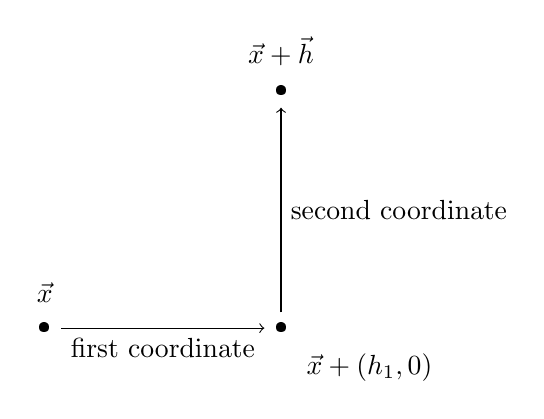
\begin{tikzpicture}
    \node[label={above:$\vec{x}$}] (a) at (0,0) {\textbullet};
    \node[label={above:$\vec{x}+\vec{h}$}] (b) at (3,3) {\textbullet};
    \node[label={below right:$\vec{x} + (h_1,0)$ }](c) at (3,0) {\textbullet};
    \path [->] (a) edge node[midway, below]{first coordinate}(c);
    \path [->] (c) edge node[midway, right]{second coordinate}(b);
    
\end{tikzpicture}
\caption{sample path for $f:\reals^2\to \reals$}
\end{figure}
On each segment of this path, $f\circ \gamma$ is a differentiable function, and we can apply the mean value theorem to bound how much $f$ changes.
\begin{proof}
It suffices to show the case where $m=1$. Let $\vec{x}\in \Omega$. We want to show that \[
Df(\vec{x}) = \begin{bmatrix}
    \pdv{f}{x_1}(\vec{x}) & \cdots & \pdv{f}{x_n}(\vec{x})
\end{bmatrix}.
\]
Let $\epsilon>0$. By continuity of the partial derivatives, find $r>0$ such that for all $1\leq j\leq n$ and $\vec{y}< r,$\[
    \left|\pdv{f}{x_j}(\vec{x}) -\pdv{f}{x_j}(\vec{x}+\vec{y}) \right| \leq \frac{\epsilon}{n}
\]
Therefore, for all $0<\vec{h}< r$,\begin{align*}
    f(\vec{x}+\vec{h}) - f(\vec{x})= & \sum_{j=1}^n f(p_j)-f(p_{j-1})\\
        \leq&\sum_{j=1}^n h_j \pdv{f}{x_j}(\tilde{p}_j),
\end{align*}
where $\tilde{p}_j$ is a point on the straight line between $p_{j-1}$ and $p_j$ by the Mean Value Theorem. Thus, 
\begin{align*}
    \frac{1}{|\vec{h}|}| f(\vec{x}+\vec{h}) - f(\vec{x}) -\begin{bmatrix}
        \pdv{f}{x_1}(\vec{x}) & \cdots & \pdv{f}{x_n}(\vec{x})
    \end{bmatrix}\vec{h}| \leq & \frac{1}{|h|}\sum_{j=1}^n |h_j| \left|\pdv{f}{x_j}(\tilde{p}_j)-
    \pdv{f}{x_j}(\vec{x})\right|\\
    \leq &\frac{1}{|h|}\sum_{j=1}^n |h| \frac{\epsilon}{n} \\
    \leq &\epsilon.
\end{align*}
We thus have \[
\lim_{\vec{h}\to\vec{0}}\frac{|f(\vec{x}+\vec{h}) - f(\vec{x}) -\begin{bmatrix}
    \pdv{f}{x_1}(\vec{x}) & \cdots & \pdv{f}{x_n}(\vec{x})
\end{bmatrix}\vec{h}|}{|\vec{h}|} = 0
\]
as desired.
\end{proof}
\theorem[chainrule]{Chain Rule}{
    Let $\Omega_1\subseteq\reals^n$, $\Omega_2\subseteq\reals^m$ be open subsets. Let $f:\Omega_1\to\Omega_2$, $g:\Omega_2\to\reals^p$ (That is, the composition $g\circ f: \Omega_1\to \reals^p$). If $f$ and $g$ are differentiable then $g\circ f$ is differentiable, and \[
        d(g\circ f) (\vec{x}) = dg(f(\vec{x})) df(\vec{x}).
    \]
}
The idea behind the proof of the chain rule is not too hard; the execution is just slightly frustrating. 
We can approximate $f$ to its first order: for some small $\Delta x$ \[
    f(\vec{x}+\Delta x)  = f(\vec{x}) + df(\vec{x}) \Delta x + \delta_f(\Delta x),
\]
with $\lim_{\Delta x\to \vec{0}} \delta_f(\Delta x) / |\Delta x| = \vec{0} $. Similarly, \[
   g( f(\vec{x})+\Delta y)  = g(f(\vec{x})) + dg(f(\vec{x})) \Delta y + \delta_g(\Delta y)
\]
with $\lim_{\Delta y\to \vec{0}} \delta_g(\Delta y) / |\Delta y| = \vec{0} $.
Therefore,\begin{align*}
    g(f(\vec{x})+ \Delta x) &= g(f(\vec{x}) + df(\vec{x}) \Delta x + \delta_f(\Delta x))\\
    &= g(f(\vec{x}))+ dg(f(\vec{x}))(df(\vec{x}) \Delta x + \delta_f(\Delta x))+\delta_g(df(\vec{x}) \Delta x + \delta_f(\Delta x))\\
    &= \textcolor{red}{g(f(\vec{x}))+ dg(f(\vec{x}))df(\vec{x}) \Delta x }+ dg(f(\vec{x}))\delta_f(\Delta x)+\delta_g(df(\vec{x}) \Delta x + \delta_f(\Delta x)).
\end{align*}
The first two terms is a linear approximation of $g\circ f$ with the `derivative' equals the product of the two matrices. Therefore, we just need to show that the remaining terms go to zero (faster than $\Delta x$) if we take the limit $\Delta x\to\vec{0}$.
\begin{proof}[Remaining part of the proof (Optional)]
    By continuity of linear transformations, we get \begin{align*}
        \lim_{\Delta x\to\vec{0}} \frac{ dg(f(\vec{x}))\delta_f(\Delta x)}{|\Delta x|} =dg(f(\vec{x}))  \lim_{\Delta x\to\vec{0}} \frac{ \delta_f(\Delta x)}{|\Delta x|} = g(f(\vec{x})) \vec{0}=\vec{0}.
    \end{align*}
    For the other term, \begin{align*}
        \lim_{\Delta x\to\vec{0}}\frac{\delta_g(df(\vec{x}) \Delta x + \delta_f(\Delta x))}{|\Delta x|} = \lim_{\Delta x\to\vec{0}}\frac{\delta_g(df(\vec{x}) \Delta x + \delta_f(\Delta x))}{|df(\vec{x}) \Delta x + \delta_f(\Delta x)|}\frac{|df(\vec{x}) \Delta x + \delta_f(\Delta x)|}{|\Delta x|}.
    \end{align*}
    By continuity of $\delta_g(df(\vec{x}) \Delta x + \delta_f(\Delta x))$ in $\Delta x$, the first term in the product goes to $\vec{0}$ as $\Delta x\to\vec{0}$. The second term is bounded by $|df(\vec{x})| + |\delta_f(\Delta x)/\Delta x|$. (Here we used $|df(\vec{x})|$ to denote the \textit{operator norm} of the matrix, which will not be tested). This term is bounded, so the magnitude of the limit is bounded by \[
        \lim_{\Delta x\to\vec{0}} C\frac{|\delta_g(df(\vec{x}) \Delta x + \delta_f(\Delta x))|}{|df(\vec{x}) \Delta x + \delta_f(\Delta x)|} = 0
    \]
    for some constant $C>0$. Therefore we get the definition of differentiability  \[
        \lim_{\Delta x\to\vec{0}} \frac{ g(f(\vec{x})+ \Delta x) - g(f(\vec{x}))- dg(f(\vec{x}))df(\vec{x}) \Delta x }{|\Delta x|}=\vec{0}.
    \]
\end{proof}
\corollary{
    Write $f(x_1,x_2,\ldots, x_n)$ and $g(y_1,y_2,\ldots, y_m)$. Then for each $1\leq k \leq n$, $1\leq l \leq m$, \[
    \frac{\partial {(g\circ f)}_l}{\partial x_k} = \sum_{i=1}^{m} \frac{\partial g_l}{\partial y_i}\frac{ \partial f_i}{\partial x_k}.
    \] 
}
\example{
    Let $f(t) = (t,t^2,t^3),w(x,y,z)=e^{xy+z}$. Compute the derivative $(w\circ f)'(t)$ using the chain rule.
}
Here we have the derivative in one varible, so this coincides with the total derivative. Moreover, these functions are elementary, so the partial derivatives are continuous (so the functions are differentaible). Using the Chain rule, \begin{align*}
    (w\circ f)'(t) &= \begin{bmatrix}
        \frac{\partial w}{\partial x}|_{(t,t^2,t^3)}&\frac{\partial w}{\partial y}|_{(t,t^2,t^3)}&\frac{\partial w}{\partial z}|_{(t,t^2,t^3)}
    \end{bmatrix}
    \begin{bmatrix}
        \frac{d t}{dt} \\ \frac{dt^2}{dt} \\ \frac{dt^3}{dt}
    \end{bmatrix} \\
    &=\begin{bmatrix}
       e^{2t^3}t^2&e^{2t^3}t&e^{2t^3}
    \end{bmatrix}
    \begin{bmatrix}
        1 \\ 2t \\ 3t^2
    \end{bmatrix}\\
    &= 6t^2 e^{2t^3}.
\end{align*}
As a sanity check, we can directily compute \[
\frac{d}{dt} w(f(t)) = \frac{d}{dt}e^{2t^3} = 6t^2e^{2t^3}
\]
using the one-dimensional chain rule you have learnt in high school calculus.
\section{Applications - Geometry of Tangent Lines and Planes }
This section will require material from the first chapter.

\example{
    Let $f:\reals^2\to\reals$ be differentiable. Find the equation of the plane tangent to the graph of $f$ at the point $(x_0,y_0,f(x_0,y_0))$.
}
The plane is the best linear approximation of $f$, \[
    f(x_0+\Delta x,y_0+\Delta y) \approx f(x_0,y_0)+ df(x_0,y_0)\begin{bmatrix}
        \Delta x \\ \Delta y
    \end{bmatrix} = f(x_0,y_0)+\frac{\partial f}{\partial x}\bigg|_{(x_0,y_0)} \Delta x + \frac{\partial f}{\partial y}\bigg|_{(x_0,y_0)} \Delta y.
\]
Therefore the tangent plane should be described by the equation \[
    z=f(x,y)+\frac{\partial f}{\partial x} (x-x_0)+\frac{\partial f}{\partial y} (y-y_0)\implies  \frac{\partial f}{\partial x} (x-x_0)+\frac{\partial f}{\partial y} (y-y_0)-(z-f(x,y))=0.
\]
\example{
    The plane tangent to the graph of $f(x,y)=x^2-y^2$ at $(1,1,0)$ is \[
           2(x-1)-2(y-1)-z=0\implies 2x-2y-z=0.
    \]
}


\definition{Directional Derivatives}{
    \domain{f}{n}{}. Let $\vec{v}\in\reals^n$. We define the \textbf{directional derivative} of $f$ along the direction of $\vec{v}$ \[
    \nabla_{\vec{v}}f (\vec{x}) \defeq \lim_{h\to0}\frac{f(\vec{x}+h\vec{v})-f(\vec{x})}{h}.
    \] 
}
\begin{remark}
In this definition, we constrain ourselves to functions $\reals^n\to\reals$. i.e. the output of the function is a scalar.
\end{remark}
\definition{Gradient}{
    \domain{f}{n}{} be differentiable. We define the \textbf{gradient} of $f$ \[
    \nabla f (\vec{x}) \defeq \begin{bmatrix}
        \frac{\partial f}{\partial x_1}\\
        \frac{\partial f}{\partial x_2}\\
        \vdots\\
        \frac{\partial f}{\partial x_n}\\
    \end{bmatrix}.
    \]
}
\begin{remark}
    Using the tranpose notation, we can also write $\nabla f$ to be the column vector ($n\times 1$ matrix) $df^T$. 
\end{remark}


\proposition{
    If $f$ is differentiable then $\nabla_{\vec{v}}f(\vec{x}) = \nabla f (\vec{x}) \cdot \vec{v}$.
}
\begin{proof}
    Since $f$ is differentaible, we have \begin{align*}
        \lim_{\vec{x}'\to\vec{x}}\frac{f(\vec{x}')-f(\vec{x})-df(\vec{x})(\vec{x}'-\vec{x})}{|\vec{x}'-\vec{x}|}=0.
    \end{align*}
    Taking this limit along the path $\vec{x}'=\vec{x}+h\vec{v}$,\begin{align*}
        0=\lim_{h\to 0}\frac{f(\vec{x}+h\vec{v})-f(\vec{x})-hdf(\vec{x})(\vec{v})}{|h||\vec{v}|}.
    \end{align*}
    Or, 
    \begin{align*}
        0&=\lim_{h\to 0}\frac{f(\vec{x}+h\vec{v})-f(\vec{x})-hdf(\vec{x})(\vec{v})}{h}\\
        &=\lim_{h\to 0}\frac{f(\vec{x}+h\vec{v})-f(\vec{x})}{h} - df(\vec{x})(\vec{v}).
    \end{align*}
    Therefore, the directional derivative is $df(\vec{x})(\vec{v}) = \nabla f(\vec{x})\cdot \vec{v}$.
\end{proof}
By the \hyperref[thm:chainrule]{Chain rule}, you should recognize this as the derivative in $t$ for the composition $f\circ \vec{r}(t)$ at $t=0$,
where $\vec{r}(0)=\vec{x}$, $\vec{r}'(0)=\vec{v}$.

In other words, suppose our $n$-th dimensional-lander Nadia is moving in $\Omega$ along a differentiable path $\vec{r}$. At the moment she reaches $\vec{x}$, her instantaneous velocity is $\vec{v}$, $\nabla_{\vec{v}}$ will be the rate of change of the $f$-meter she experiences. 

\example{
    \domain{f}{n}{} be differentiable. Suppose that $\nabla f (\vec{x})\neq \vec{0}$.
    Find the unit vector $\vec{u}$ such that $\nabla_{\vec{u}}$ is i) largest, ii) smallest.
}
In other words, suppose Nadia is now moving with unit speed. What direction does she need to face for the fastest ascent/descent of the $f$-meter?

By the \hyperref[thm:cauchyschwarz]{Cauchy Schwarz inequality}, we get \[
|\nabla_{\vec{u}}f (\vec{x})| \leq |\nabla f||\vec{u}| = |\nabla f|.
\]
Therefore, the best we can hope for is a rate of $|\nabla f|$ for ascent or a rate of $-|\nabla f|$ for descent. Fortunately, this is possible with the following unit vectors: \begin{align*}
    \nabla f \cdot \frac{\nabla f}{|\nabla f|} &= |\nabla f|,\\
    \nabla f \cdot \frac{-\nabla f}{|\nabla f|}&= -|\nabla f|.
\end{align*}
This means that $\nabla f$ also points in the direction of fastest ascent, and the magnitude of $\nabla f$ describes the rate of ascent! 
\begin{remark}
    You can also see ${\nabla f} $ and $ -\nabla f$ will form an angle of $0$ or $\pi$ with $\nabla f$, so you can also construct these two unit vectors using the cosine definition of dot product.
\end{remark}
\begin{aexample}{Level sets orthogonal to gradient}{}
    Show that levels sets are orthogonal to the gradient. Precisely, let $\Omega\subset \reals^n$, $f:\Omega \to \reals$$\gamma:[0,1]\to \Omega$ be a curve that satisfies \[
    f(t)=c
    \]
    for a constant $c$. Show that \[
        \gamma'(t) \cdot (\nabla f)(\gamma(t))=0.
    \]
    for all $t\in [0,1]$. Here \[
    \gamma'(t) \defeq D\gamma(t) = \begin{bmatrix}
        \gamma_1'(t)\\\vdots\\\gamma_n'(t)
    \end{bmatrix}.
    \]
\end{aexample}
We apply the Chain rule on the function $f(\gamma(t))$.
On one hand, since $f(\gamma(t))$ is constant, \[
D(f\circ \gamma) (t) = 0.
\]
Using the chain rule, \[
    D(f\circ \gamma) (t) = (Df)(\gamma(t)) \gamma'(t) = (\nabla f)(\gamma(t)) \cdot \gamma'(t).
\]
\example{
    Consider the level set of the function \[
    F(x,y,z)=xy-z
    \]
    at $0$. What is the equation of the tangent plane of the level set at $(0,0,0)$.
}

At the origin, $\nabla F = (0,0,1)$. This vector is normal to the level set, that is, it is normal to the tangent plane of the level set at $(0,0,0)$, therefore, the equation of the tangent plane is \[
0(x-0) + 0(y-0) + 1(z-0) = 0 \implies z=0.
\]
The tangent plane is the $xy$-plane. You can confirm that the level set is the graph of the function $z=xy$. This is the \hyperref[saddle]{saddle} we graphed a few sections ago. At the origin, the saddle is locally flat, so has the flat tangent plane.
\section{Implicit Differentiation}
We warmup with an example of implicit differentiation in one variable.
\example{
    Let $x^2+y^2=1$. Find $dy/dx$.
}
To solve this, we can take the derivative with respect to $x$ on both sides to get \[
2x+2y \frac{dy}{dx}=0 \implies \frac{dy}{dx}=-\frac{x}{y}.
\]
Let us interpret the result as a sanity check. $x^2+y^2=1$ describe a circle, and $dy/dx$ is the slope of the tangent line at any point. At $(0,1)$ and $(0,-1)$, we get the highest and lowest points of the circle, so the slope is $0$. In the first and third quadrant, the slope is negative; in the second and fourth quadrant, the slope is positive.

This $dy/dx$ seems slightly different from the usual limit definition in the sense that $y$ is not necessarily a function of $x$. However, we can locally define $y$ in terms of $x$ as follows. \begin{itemize}
    \item In the top half plane where $y>0$, we can set $y=\sqrt{1-x^2}$.
    \item In the top half plane where $y<0$, we can set $y=-\sqrt{1-x^2}$.
\end{itemize}
Under this construction, you can verify that $dy/dx=-x/y$ at any point on the circle where $y\neq 0$. When $y=0$, the function breaks down as we divide by zero. This corresponds to the vertical tangent line at that point. There is no way to define $y$ locally as a function of $x$. 

\begin{figure}[h]
    \centering
    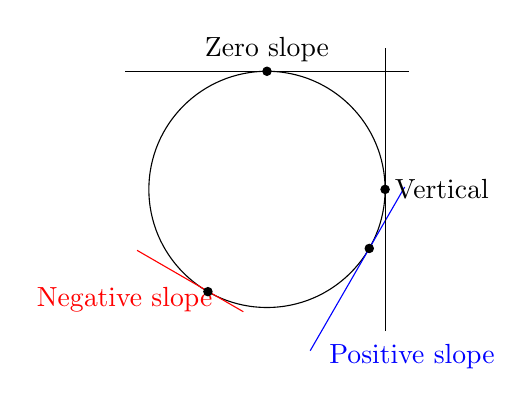
\begin{tikzpicture}[scale=1.5]
        % Draw unit circle
        \draw (0,0) circle (1);
      
        % Zero slope tangent at (0,1)
        \draw (-1.2,1) -- (1.2,1) node[above,midway] {Zero slope};
      
        % Positive slope tangent in fourth quadrant (0.866, -0.5)
        \draw[blue] (0.866 - 0.5, -0.5 - 0.866) -- 
                    (0.866 + 0.3, -0.5 + 0.520) 
                    node[below right , pos=0.1] {Positive slope};
      
        % Negative slope tangent in third quadrant (-0.5, -0.866)
        \draw[red] (-0.5 - 0.6, -0.866 + 0.35) -- 
                   (-0.5 + 0.3, -0.866 - 0.17) 
                   node[left, pos=0.8] {Negative slope};
      
        % Vertical tangent at (1,0)
        \draw (1,-1.2) -- (1,1.2) node[right,midway] {Vertical};
      
        % Add reference points
        \filldraw (0,1) circle (1pt) (1,0) circle (1pt)
                  (0.866,-0.5) circle (1pt) (-0.5,-0.866)  circle (1pt);
      \end{tikzpicture}
    \caption{We can define $y$ as a function of $x$ locally on the level set $x^2+y^2=1.$}
\end{figure}
The way we defined $y$ as a function of $x$ is known as an implicit function. In the sense that it is implicitly defined by the equation $x^2+y^2=1$.
\definition{Implicit Equation}{
    \domain{f}{n}{m}. An \textbf{implicit equation} is a relation in the form\[
    f(\vec{x})=\vec{0}.
    \]
    By defining $g(\vec{x})=f(\vec{x})-\vec{c}$ for some constant $\vec{c}\in \reals^m$, we also get\[
    f(\vec{x})=\vec{c} 
    \]
    is an implicit equation.
}
Our question is as follows: given an implicit equation, can we `solve' this equation locally? If such an equation exists, what is the partial derivatives of the variables?

We shall spoil the big result of this section. 
\begin{atheorem}{Implicit function}{implicitfunction}
    \domain{f}{n+m}{n}. We denote the coordinates of a point $(\vec{x},\vec{y})\in \Omega$ as $(x_1,x_2,\ldots, x_n,y_1,\ldots,y_m)$. Let $(\vec{a},\vec{b})\in \Omega$. If the matrix \[
    \begin{bmatrix}
        \pdv{f_1}{x_1} & \pdv{f_1}{x_2} & \cdots & \pdv{f_1}{x_n}\\
        \vdots &\ddots&& \vdots \\
         \pdv{f_n}{x_1}& \pdv{f_n}{x_2} &\cdots & \pdv{f_n}{x_n}
    \end{bmatrix}
    \] is invertible at $(\vec{a},\vec{b})\in \Omega$, then there exists an open set $U\subseteq \reals^m$ containing $\vec{b}$ and a differentiable function $g:U\to \reals^n$ such that \[
    f(g(\vec{y}),\vec{y})
    \]
    is constant, and $g(\vec{b})=\vec{a}$. In this case, we call the function $g$ an \textbf{implicit function}.
\end{atheorem}

Before we work through some examples, let us parse the statement of the Implicit Function Theorem. 
The Jacobian matrix of $f$ can be expressed as \[
    Df\defeq \begin{bmatrix}[c | c]
        Df_x&Df_y
    \end{bmatrix}.= \begin{bmatrix}[c c c c | c c c c]
        \pdv{f_1}{x_1} & \pdv{f_1}{x_2} & \cdots & \pdv{f_1}{x_n}& \pdv{f_1}{y_1} & \pdv{f_1}{y_2} & \cdots & \pdv{f_1}{y_m}\\
        \vdots &\ddots&& \vdots & \vdots &\ddots&& \vdots \\
        \pdv{f_n}{x_1}& \pdv{f_n}{x_2} &\cdots & \pdv{f_n}{x_n}&\pdv{f_n}{y_1}& \pdv{f_n}{y_2} &\cdots & \pdv{f_n}{y_m}
    \end{bmatrix}.
\]
This is a $n\times(n+m)$ matrix. The left matrix $Df_x$ is exactly the matrix we want to check for the conditions of Implicit Function theorem. If it is invertible, then That One Theorem implies that there is a unique solution in $\vec{x}$ for the equation \[
    Df_x \vec{x} + Df_y\vec{y}= \vec{c}
\]
for any fixed $\vec{c}\in \reals^n$ and $\vec{y}\in \reals^m$. Therefore, if we hold $\vec{c}$ constant, we should expect that we can solve $\vec{x}$ as a function of $\vec{y}$. 

Another way to look at it is to apply the Rank-Nullity theorem. Approximating the function locally as \[
    f(\vec{a},\vec{b})+Df_x(\vec{x}-\vec{a})+Df_y(\vec{y}-\vec{b})+ \rm{error}.
    \]
The rank of $Df$ is $n$, so the nullity is $(n+m)-n= m $. We thus have $m$ dimensions that are in `excess'. These $m$ variables are the $y_j$'s, each corresponding to one dimension in the nullspace of $D_f$. 

\begin{aexample}{Derivative of implicit function}{implicitjacobian}
    Work out the derivative of the implicit function $g:U\to \reals^n$ using the Chain rule.
\end{aexample}

Recall that $f(g(\vec{y}),\vec{y})$ is constant. This is a composition of two functions. The first function sends \[
\vec{y}\mapsto (g(\vec{y}),\vec{y}),
\]
which has Jacobian matrix \[
    \begin{bmatrix}
        Dg \\\hline I_m
    \end{bmatrix}
\]
and the second function is $f$. Since the function is constant, the derivative of the composition of these functions is $0_{m\times m}$, so we have \[
    0_{m\times m}=
    \begin{bmatrix}[c | c]
        Df_x&Df_y
    \end{bmatrix} \begin{bmatrix}
        Dg \\\hline I_m
    \end{bmatrix} = Df_xDg + Df_y.
\]
Rearranging the terms,\[
    -Df_y = Df_xDg \implies Dg = -Df_x^{-1}Df_y.
\]


\example{\domain{f}{n}{}. Suppose for $\vec{v}\in \Omega$ satisfies $\nabla f (\vec{v})\neq \vec{0}$. What is the local dimension of the level set described by the implicit equation\[
    f(\vec{x})=f(\vec{v})
\]
around $\vec{v}$?
}
We wish to apply the implicit function theorem. If the conditions of the implicit function theorem applies, then this will be a function $\reals^{(n-1)+1} \to \reals^1$. So the implicit function gives that the level set is locally the graph of a function in $(n-1)$ variables (locally $(n-1)$ dimensions).

To check for the conditions of implicit function theorem, we use the fact that $Df = \nabla f^T$ is non zero at $\vec{v}$, thus has rank $1$. If the $i$-th column is the pivot column, then we can express \[
x_i = g(x_1,x_2,\ldots, x_{i-1},x_{i+1},\ldots, x_n)
\]  

Physically, $Dg$ will define the tangent line/plane/hyperplane to the level set at $(\vec{v},f(\vec{v}))$.

The tangent plane is not guaranteed to exist. For instance, take the implicit equation described by \[
    x^2-y^2=0.
\]
Plotting this in $\reals^2$, this gives two lines $y=x$ and $y=-x$. At almost every point $(x,y)$ in the level set, exactly one of $y=x$ or $y=-x$ hold. Therefore, we can restrict our attention to one line, and the local dimension of the line is $1$.

On the other hand, the point $(0,0)$ lies on both lines. For a (miniature-sized) person standing at the origin, the level set is locally a cross, which is the union of two $1$-dimensional objects does not look like a line or a plane.

by the Implicit Function Theorem. 
\definition{Implicit Derivative}{
    \domain{f}{n}{}. Consider the implicit equation \[
        f(\vec{x})= c.
    \]We define the \textbf{Implicit Derivative} \[
    \frac{\partial x_i}{\partial x_j} \defeq \frac{\partial g}{\partial x_j},
    \]
    where $g$ is the implicit function that solves for $x_i$ using the variables $(x_1,\ldots,x_{i-1},x_i,\ldots, x_n)$.
}
\example{
    Express the implicit derivative in terms of the partial derivatives of $f$.
}
We first check the conditions of the Implicit function theorem. To express $x_i$ as an implicit function of the other variables, the square `matrix' we need to check for invertibility is \[
\begin{bmatrix}
    \pdv{f}{x_i}
\end{bmatrix}.
\]
This is invertible exactly when the partial derivative is non zero. Thus using Example \ref{ex:implicitjacobian}, \[
\pdv{x_i}{x_j}= -\frac{\pdv{f}{x_j}}{\pdv{f}{x_i}}.
\]
You can confirm this equation for $dy/dx$ on the circle implicitly defined by $x^2+y^2=1$.

\section{Inverse function theorem}
We can also ask the question of whether a function has an inverse. That is, for a function $f:\reals^n\to\reals^m$, is there a function $g:\reals^m\to\reals^n$ that undos $f$. We require \[
    f(g(\vec{y})) = \vec{y} 
\]
for all $\vec{y}\in\reals^m$ and \[
g(f(\vec{x}))=\vec{x}
\]
for all $\vec{x}\in \reals^n$. If such a function exists, we call it the inverse of $f$, and denote it as $f^{-1}$.

\example{
    Suppose $f^{-1}$ exists. What is $D(f^{-1})$?
}

We apply the chain rule on $f\circ f^{-1}$ and $f^{-1}\circ f$. Suppose $f(\vec{x})=\vec{y}$ and thus $f^{-1}(\vec{y})=\vec{x}$.
On one hand, we have \[
I_m=D(f\circ f^{-1})(\vec{y}) = Df (f^{-1}(\vec{y})) D(f^{-1})(\vec{y})= Df (\vec{x}) D(f^{-1})(\vec{y}).
\]
On the other hand, we have \[
    I_n=D(f\circ f^{-1}) = D(f^{-1}) (f(\vec{x})) Df(\vec{x})= D(f^{-1}) (\vec{y}) Df(\vec{x}).
\]
That means $Df(\vec{x})$ has a left and right inverse $D(f^{-1})(\vec{y})$. So $Df(\vec{x})$ is surjective and injective by Example \ref{ex:ex:leftrightsurinj}. By That One Theorem, $Df(\vec{x})$ is invertible, with $(Df(\vec{x}))^{-1}=D(f^{-1})(\vec{y})$.

The surprising fact is that the converse is true. If $Df(\vec{x})$ is invertible, then locally there is an inverse function $f^{-1}$.
\theorem{Inverse Function}{
    \domain{f}{n}{n}. Let $\vec{a}\in\Omega$, and suppose that $Df(\vec{x})$ is invertible. Then there exists open sets $U$ containing $\vec{a}$ and $V$ containing $\vec{b}=f(\vec{a})$, and a function $g:V\to U$ such that \begin{align*}
        f(g(\vec{y}))&=\vec{y}\\
        g(f(\vec{x}))&=\vec{x}
    \end{align*}
    for all $\vec{y}\in V$ and $\vec{x}\in U$.
    Moreover, \[
    Dg(\vec{y}) = (Df(\vec{x}))^{-1} 
    \]
    for $\vec{y}=f(\vec{x})$, and $\vec{x}\in U$.
}
\begin{proof}
    The second statement is a result of the previous example, so we only need to show the first statement. 

    Consider the implicit equation in $2n$ variables \[
    f(\vec{x}) -\vec{y}=\vec{0}.
    \]
    On one hand, we can solve $\vec{y}=f(\vec{x})$ explicitly. By the inverse function theorem, this is unique at some open set around $\vec{x}$. If we can obtain $\vec{x} = g(\vec{y})$ as an implicit function, then we must have $f$ and $g$ are inverses of each other. Indeed, since $Df$ is invertible, the conditions of the Implicit Function Theorem apply and we have an implicit function $g$ such that \[
    f(g(\vec{y}))-\vec{y}=\vec{0}.
    \]
\end{proof}
\exercises
